\section{Felder}
\textbf{Materialgleichungen}
\begin{align*}
    \Aboxed{\vec{J}  = \kappa\vec{E} = \left[\dfrac{A}{m^2}\right]} &
    \Aboxed{\vec{B}  = \mu\vec{H} = [T]}    &
    \Aboxed{\vec{D}  = \varepsilon\vec{E} = \left[\dfrac{C}{m^2}\right]}
\end{align*}

Verkopplung von $ \vec{E}$- und $ \vec{H}$-Felder über $ \vec{J}=\kappa\vec{E}$.\\

\textbf{Feldunterscheidung}
\begin{align*}
     & \vec{E}(x,y,z)                               & \widehat= & \quad\text{statisches Feld}  & \\
     & \vec{E}(x,y,z,t)                             & \widehat= & \quad\text{stationäres Feld} & \\
     & \vec{E}(x,y,z,t)\cdot cos(\omega t -\beta z) & \widehat= & \quad\text{Welle}            &
\end{align*}


%\subsection{E-Felder an Grenzflächen}
%\textbf{Dielektrische Grenzfläche}\\
%\begin{tabularx}{0.45\textwidth}{>{\hsize=.3\hsize}X>{\hsize=.5\hsize}X}
%    Querschichtung:   & $D_{1n} = D_{2n}$                                                                                                        \\
%                      & ${\displaystyle\oiint} \vec{D} \cdot d \vec{a} = 0$                                                                      \\
%    Längsschichtung:  & $E_{1t} = E_{2t}$                                                                                                        \\
%                      & $ {\displaystyle\oint} \vec{E} \cdot d \vec{s} = 0$                                                                      \\
%    Schrägschichtung: & $ \frac{\tan( \alpha_1)}{\tan( \alpha_2)} = \frac{E_{1t}/E_{1n}}{E_{2t}/E_{2n}} = \frac{ \varepsilon_1}{\varepsilon_2} $
%\end{tabularx}
%
%\textbf{Grenzfläche dielektrischer Leiter}\\
%\begin{tabularx}{0.45\textwidth}{>{\hsize=.3\hsize}X>{\hsize=.5\hsize}X}
%    Längsschichtung: & $E_{1t} = E_{2t}$                                   \\
%                     & ${\displaystyle\oint} \vec{E} \cdot d \vec{s} = 0$  \\
%    Querschichtung:  & $D_{1n} = \frac{Q}{A}$                              \\
%                     & ${\displaystyle\oiint} \vec{D} \cdot d \vec{a} = Q$
%\end{tabularx}
%
%\textbf{Grenzfläche an magn. Feldern}\\
%\begin{tabularx}{0.45\textwidth}{>{\hsize=.3\hsize}X>{\hsize=.5\hsize}X}
%    Querschichtung:   & $B_{1n} = B_{2n}$                                                    \\
%                      & ${\displaystyle\oiint} \vec{B} \cdot d \vec{a} = 0$                  \\
%    Längsschichtung:  & $H_{1t} = H_{2t}$                                                    \\
%                      & ${\displaystyle\oint} \vec{H} \cdot d \vec{s} = 0$                   \\
%    Schrägschichtung: & $\frac{\tan( \alpha_1)}{\tan( \alpha_2)} = \frac{ \mu_1 }{ \mu_2 } $
%\end{tabularx}

\subsection{Elektrostatik}
%\textbullet wirbelfreie Felder $\rightarrow$ Skalarpotenzial $\rightarrow$ Elektrische Ladungen sind Quellen des
%Feldes

%\begin{align*}
%    \Aboxed{\opdiv \vec{D} & = \nabla \cdot \vec{D}  = \rho} & \qquad \vec{D} & = \varepsilon \vec{E} \\
%    \Aboxed{\oprot \vec{E} & = \nabla \times \vec{E} = 0}    & \qquad         & = \oprot \opgrad E\\
%    \vec{E} & = - \opgrad \varphi 
%\end{align*}

Wirbelfreie Felder $\rightarrow$ Gradientenfeld $\rightarrow$ elek. Ladungen sind Quellen des $\vec{E}$-Feldes (Skalare Potenzialfkt. $ \varphi $)
\begin{align*}
	\oprot \vec{E} & = 0 = \oprot \opgrad E & \vec{E} & = -\opgrad \varphi &\\
	\opdiv \vec{D} & = \rho & \vec{D} & = \varepsilon \vec{E} &
\end{align*}
\begin{equation*}
	\vec{E} = -\opgrad \varphi = - \left( \tfrac{\partial \varphi}{\partial x}\right) \vec{e}_x - \left( \tfrac{\partial \varphi}{\partial y}\right) \vec{e}_y - \left( \tfrac{\partial \varphi}{\partial z}\right) \vec{e}_z
\end{equation*}

%\textbf{$\qquad \Rightarrow$ Poisson-Gleichung} mit $\rho = 0$
%$\rightarrow$ \textbf{Laplace-Gleichung}

\subsubsection{Potential-/Poisson-Gleichung}
%Annahme: $ \varepsilon_r = \mathtt{konst.} $\\
La-Place-Gleichung, wenn $ \rho = 0 $
%\[
%    \opdiv \opgrad \varphi = \Delta \varphi = - \dfrac{\rho}{\varepsilon}
%\]e
\begin{align*}
	\opdiv \opgrad \varphi = \Delta \varphi  &= - \dfrac{\rho}{\varepsilon}\\
    \Delta \varphi + \underbrace{ \dfrac{\opgrad \varepsilon \cdot \opgrad \varphi}{\varepsilon}}_{= 0\texttt{, wenn homogen}}
     & = - \dfrac{\rho (x, y, z)}{\varepsilon} \\
    \frac{d^2 \varphi}{d x^2} + \frac{d^2 \varphi}{d y^2} + \frac{d^2 \varphi}{d z^2}
     & = - \dfrac{\rho (x, y, z)}{\varepsilon}
\end{align*}

\textit{Vereinfachung} zu 1-dimensionalem System:
\begin{align*}
	\text{z.B. mit}\, \frac{\partial^2...}{\partial y^2} = \frac{\partial^2...}{\partial z^2} = 0 \quad \Rightarrow \, \frac{\partial^2 \varphi}{\partial x^2} = -\frac{\rho}{\varepsilon}
\end{align*}
%z.B. mit $ \frac{\partial^2...}{\partial y^2} = \frac{\partial^2...}{\partial z^2}=0 $

\subsubsection{Randwertprobleme, -bedingungen (RB)}
%\begin{tabularx}{0.45\textwidth}{>{\hsize=.3\hsize}X|>{\hsize=.7\hsize}X}
%	Dirichlet-RB &Gesuchte Potenzialfunktion $ \varphi $ nimmt an den Rändern einen bestimmten Wert an (Bsp.: $\rho_r = 5V$) \\
%	\hline
%	Neumann-RB   & Die Normalenableitung $ \tfrac{\partial\varphi}{\partial n} $ der Fkt. $ \varphi $ nimmt an den Rändern einen bestimmten Wert an. (Bsp.: Grenzfläche unterschiedlicher Dielektrika)   \\
%\end{tabularx}
	\textbf{Dirichlet-RB}: Gesuchte Potenzialfunktion $ \varphi $ nimmt an den Rändern einen bestimmten Wert an (Bsp.: $\rho_r = 5V$) \\
	
	\textbf{Neumann-RB}: Die Normalenableitung $ \tfrac{\partial\varphi}{\partial n} $ der Fkt. $ \varphi $ nimmt an den Rändern einen bestimmten Wert an. \\ (Bsp.: Grenzfläche unterschiedlicher Dielektrika)

\subsubsection{Green'sche Funktionen}
\textbullet{\textbf{Skalarpotential} einer Punktladung}
\[ \varphi (r) = \dfrac{Q}{4 \pi \varepsilon_0 \cdot r} \qquad\left[V\right]\] 

\textbullet{\textbf{E-Feld} einer Punktladung}
\[ \vec{E}(r) = \dfrac{Q}{4 \pi \varepsilon_0 \cdot r^2}\cdot\vec{e}_r \qquad\left[\frac{V}{m}\right]\] 

\textbullet{\textbf{D-Feld} einer Punktladung}
\[ \vec{D}(r) = \dfrac{Q}{4 \pi \cdot r^2}\cdot\vec{e}_r \qquad\left[\frac{As}{m^2}=\frac{C}{m^2}\right]\]

\textbullet{\textbf{Potentialfeld} einer Ladungsdichteverteilung}

mit $\varphi(\infty)=0$
\[
    \varphi(x, y, z)=\frac{1}{4 \pi \varepsilon} \iiint_{V^{\prime}}
    \frac{\rho\left(x^{\prime}, y^{\prime},
        z^{\prime}\right)}{\left|\vec{r}-\vec{r}^{\,\prime}\right|} \mathrm{d}
    V^{\prime}
\]

mit der Green'schen Funktion $G\left(\vec{r}, \vec{r}^{\,\prime}\right)=\frac{1}{4 \pi \varepsilon\left|\vec{r}-\vec{r}^{\,\prime}\right|}$
\[\varphi(x, y, z)=\iiint_{V^{\prime}} G\left(\vec{r}^{\,\prime} \vec{r}^{\,\prime}\right) \rho\left(\vec{r}^{\,\prime}\right) \mathrm{d} V^{\prime}\]

\subsubsection{Elektrischer Dipol}
Dipolmoment $\vec{p} = Q\cdot\vec{d}$

\makebox[0pt][l]{
	\begin{minipage}[b]{0.5\columnwidth}
		\usetikzlibrary{calc, positioning}
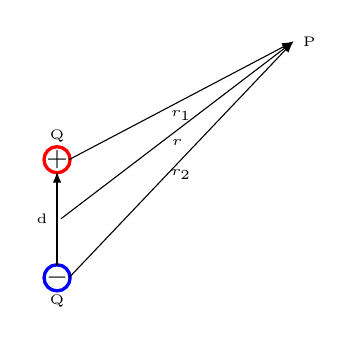
\begin{tikzpicture}[
        circ/.style = {circle, draw, minimum size =3mm, node contents={}}
    ]
    %Kreise
    \node (neg_pol)[circ, very thick, blue];
    \node at(0,0)[]{$-$};
    \node at(0,-0.1)[below]{\tiny{Q}};

    %Kreise
    \node at(0,1.5)(pos_pol)[circ, very thick, red];
    \node at(pos_pol.center)[]{$+$};
    \node at(0,1.6)[above]{\tiny{Q}};


    %Pfeile
    \draw[-latex] (0,0.15)      -- (0,1.35) node[left, midway]{\tiny{d}};
    \draw[-latex] (0.15,1.5)    -- (3,3) node[midway, below]{\tiny{$r_1$}};
    \draw[-latex] (0.05,0.75)   -- (3,3) node[right]{\tiny{P}} node[midway, below]{\tiny{$r$}};
    \draw[-latex] (0.15,0)      -- (3,3) node[midway, below]{\tiny{$r_2$}};


    %Legende

\end{tikzpicture}


	\end{minipage}
	\begin{minipage}[b]{0.5\columnwidth}
		\usetikzlibrary{calc, positioning}
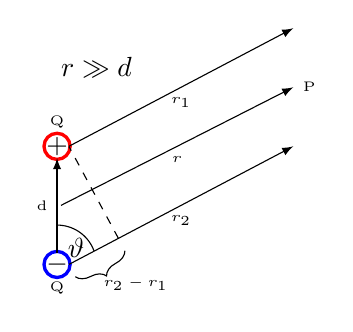
\begin{tikzpicture}[
    circ/.style = {circle, draw, minimum size =3mm, node contents={}}
]
    %Kreise
    \node (neg_pol)[circ, very thick, blue];
    \node at(0,0)[]{$-$};
    \node at(0,-0.1)[below]{\tiny{Q}};

    %Kreise
    \node at(0,1.5)(pos_pol)[circ, very thick, red];
    \node at(pos_pol.center)[]{$+$};
    \node at(0,1.6)[above]{\tiny{Q}};

    %Pfeile
    \draw[-latex] (0,0.15) -- (0,1.35)
    node[left, midway]{\tiny{d}};
    \draw[-latex] (0.15,1.5) -- (3,3)
    node[midway, below]{\tiny{$r_1$}};
    \draw[-latex] (0.05,0.75) -- (3,2.25)
    node[right]{\tiny{P}}
    node[midway, below]{\tiny{$r$}};
    \draw[-latex] (0.15,0) -- (3,1.5)
    node[midway, below]{\tiny{$r_2$}};

    %gestrichelte Linie
    \draw[dashed](0.78,0.33) -- (0.15,1.5);

    %Winkel
    \draw[-] (90:0.5) arc (90:20:0.5)
    node[left, yshift=1] {$\vartheta$};

    %Klammer
    \draw [black,
        decorate,
        decoration = {brace,
                raise=5pt,
                amplitude=5pt}] (0.78,0.33) -- (0.15,0);
    \node at (1,-0.25) []{\tiny{$r_2-r_1$}};
    %Legende
    \node at(0.5,2.5){$r\gg d$};

\end{tikzpicture}

	\end{minipage}
}

\makebox[0pt][l]{
	\begin{minipage}[]{0.5\columnwidth}
		\begin{align*}
			\varphi & = \frac{Q}{4\pi\varepsilon_0}\left(\frac{1}{r_1}-\frac{1}{r_2}\right)                                        \\
			& = \frac{Q}{4\pi\varepsilon_0}\cdot\frac{r_2-r_1}{r^2}                                                        \\
			\vec{E} & = -\nabla\varphi                                                                                             \\
			& = \frac{1}{4\pi\varepsilon_0}\cdot\left(\frac{3(\vec{p}\cdot\vec{r})\vec{r}}{r^5}-\frac{\vec{p}}{r^3}\right)
		\end{align*}
	\end{minipage}
	
	\begin{minipage}[]{0.5\columnwidth}
		\begin{align*}
			\varphi & \approx\frac{Qd\cos\theta}{4\pi\varepsilon_0r^2}                  \\
			& = \frac{1}{4\pi\varepsilon_0}\cdot\frac{\vec{p}\cdot\vec{r}}{r^3}
		\end{align*}
	\end{minipage}
}

\subsection{Magnetostatik}
Quellenfreie Wirbelfelder mit \textit{geschlossenen} Feldlinien.\\
Keine magnetischen Monopole: $\opdiv \vec{B} = 0$.\\
Skalarpotential $ \varphi_m$ existiert, wenn $\vec{H}$ wirbelfrei ist:\\
$\oprot \vec{H} = 0$, wenn $ \vec{J}=0$. 
%\textbullet Vektorpotential $ \vec{A}$ = Maß für $\Phi_{magn} $ durch Fläche A
\begin{align*}
	\opdiv \vec{B} & = 0 = \opdiv \oprot B & \vec{H} & = -\opgrad \varphi_m &\\
	\oprot \vec{H} & = \vec{J} & \vec{B} & = \mu \vec{H} &
\end{align*}
%\begin{align*}
%    \Aboxed{\oprot \vec{H} = \nabla \times \vec{H} & = \vec{J} }          & \vec{B} & = \mu \vec{H}           \\
%    \vec{H}                                        & = - \nabla \varphi_m &                                   \\
%    \Aboxed{\opdiv \vec{B} = \nabla \cdot \vec{B}  & = 0 }                &         & = \opdiv \oprot \vec{B}
%\end{align*}
\subsubsection{Vektorpotential}
Reine Hilfsgröße, in Analogie zum elek. Skalarpotential $ \varphi $.\\
\textbf{Coulomb-Eichung}, wenn $ \opdiv \vec{A} = 0 $, gilt nur für zeitunabhängige Felder.
\begin{align*}
    \Delta \vec{A} & = - \mu \vec{J} &
    \vec{B}        & = \oprot \vec{A} &
\end{align*}

\subsubsection{Vektorpotential in Abhängigkeit von der Stromdichte}
\[
    \vec{A}(x, y, z)=\frac{\mu}{4 \pi} \iiint_{V^{\prime}} \frac{\vec{J}\left(x^{\prime}, y^{\prime}, z^{\prime}\right)}{\left|\vec{r}-\vec{r}^{\,\prime}\right|} d V^{\prime}
\]

\subsubsection{Biot-Savart-Gesetz}
\[
    \vec{H}=\frac{I}{4 \pi} \oint_{C^{\prime}} \opgrad \frac{1}{\left|\vec{r}-\vec{r}^{\,\prime}\right|} \times \mathrm{d} \vec{s}^{\,\prime}
\]

mit $\opgrad \frac{1}{\left|\vec{r}-\vec{r}^{\,\prime}\right|}=-\frac{\vec{r}-\vec{r}^{\,\prime}}{\left|\vec{r}-\vec{r}^{\,\prime}\right|^{3}}$

\[
    \vec{H}=\frac{I}{4 \pi} \oint_{C^{\prime}} \frac{\mathrm{d} \vec{s}^{\,\prime} \times\left(\vec{r}-\vec{r}^{\,\prime}\right)}{\left|\vec{r}-\vec{r}^{\,\prime}\right|^{3}}
\]

{\footnotesize$\vec{r}:$ Aufpunkt $\quad \vec{r}^{\,\prime}:$ Quellpunkt}

\subsubsection{Magnetischer Dipol}
\usetikzlibrary{shapes.geometric}
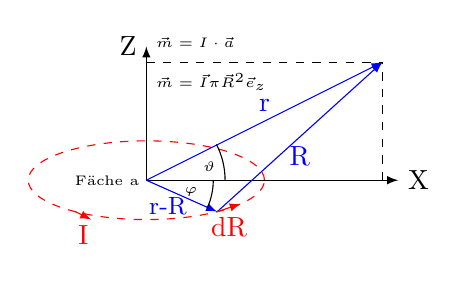
\begin{tikzpicture}
    %Elipse
    \node[ellipse,
        draw = red,
        dashed,
        minimum width = 3cm,
        minimum height = 1cm] (e) at (0,0) {};
    %Koordinaten Achsen
    \draw[-latex](0,0)--(3.2,0) node[right]{X};
    \draw[-latex](0,0)--(0,1.7) node[left]{Z};
    %Pfeile
    \draw[-latex, blue](0,0)--(3,1.5) node[above, midway]{r};
    \draw[-latex, blue](0.9,-0.4)--(3,1.5) node[below, midway]{R};
    \draw[-latex, blue](0,0) -- (0.9,-0.4) node[midway, below, yshift=3pt, xshift=-5pt]{\small{r-R}};
    \draw[-latex, red](0.9,-0.4)--(1.2,-0.3) node[midway, below]{dR};
    \draw[-latex, red](-0.9,-0.4)--(-0.7,-0.5) node[midway, below]{I};
    %Winkel
    \draw[-] (27:1) arc (27:0:1)
        node[left, yshift=5] {\tiny{$\vartheta$}};
    \draw[-] (0:0.85) arc (0:-25:0.85)
        node[left, yshift=6] {\tiny{$\varphi$}};
    %Legende
    \node[right] at (0,1.25){\tiny{$\vec{m}=\vec{I}\pi\vec{R}^2\vec{e}_z$}};
    \node[right] at (0,1.75){\tiny{$\vec{m}=I\cdot\vec{a}$}};
    \node[] at (-0.5,0){\tiny{Fäche a}};
    %Linien
    \draw[dashed](3,0)--(3,1.5);
    \draw[dashed](0,1.5)--(3,1.5);
\end{tikzpicture}
\\
I entlang eines Leiters:
\begin{align*} 
    A(r)                            & = \frac{\mu_0 \cdot I}{4 \pi} \int \frac{d \vec{s}}{| \vec{r} - \vec{s}|} = \frac{ \mu_0}{4 \pi} \frac{\vec{m} \times \vec{r}}{r^3} \\
    \vec{B} = \nabla \times \vec{A} & = \frac{\mu_0}{4 \pi} \left(\frac{3(\vec{m} \cdot \vec{r})\vec{r}}{r^5} - \frac{\vec{m}}{r^3}\right)
\end{align*}

\subsection{Quasistätionäre Felder (Wechselstrom)}
Homogenes, Isotropes Medium: $ \varepsilon, \mu, \kappa = \mathtt{kost.} $\\
Leiter ist quasineutral: $ \rho = 0 $.
\begin{align*}
	\oprot \vec{E} & = -\frac{\partial \vec{B}}{\partial t} = -\mu \frac{\partial \vec{H}}{\partial t} & \opdiv \vec{E} & = 0 & \vec{D}  &= \varepsilon\vec{E} & \\
	\oprot \vec{H} & = \vec{J} = \kappa \vec{E} & \opdiv \vec{B} & = 0 &\vec{B}  &= \mu\vec{H}&\\
	\opdiv \vec{J} &= -\frac{\partial \rho}{\partial t}& \opdiv \vec{H} &= 0 & \vec{J} &= \kappa \vec{E}&
\end{align*}
%\begin{align*}
%	\opdiv \vec{B} & = 0 = \opdiv \oprot B & \vec{H} & = -\opgrad \varphi_m &\\
%	\oprot \vec{H} & = \vec{J} & \vec{B} & = \mu \vec{H} &
%\end{align*}

\subsubsection{Komplexe Feldgrößen}
\textbullet komplexe Amplitude / Phasor:
\begin{equation*}
	\underline{J}=J\cdot e^{j\varphi}
\end{equation*}
\textbullet komplexer Amplituden-Drehzeiger:
\begin{align*}
\underline{J}(t)&=\underline{J} \cdot e ^{jwt} = J \cdot e^{j(wt+\varphi)}
\end{align*}
\textbullet Darstellung in karthesischen Koordinaten:
\begin{align*}
	\underline{J}&=\underline{J}_x \cdot \vec{e}_x + \underline{J}_y \cdot \vec{e}_y + \underline{J}_z \cdot \vec{e}_z
\end{align*}

\subsubsection{Skineffekt}

\begin{center}
    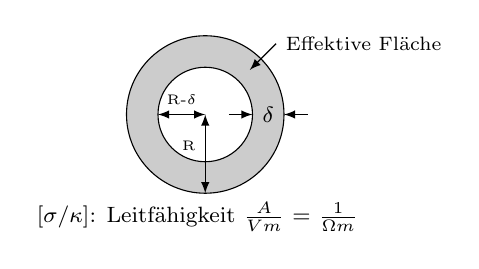
\begin{tikzpicture}
        %Kreise
        \draw[-,fill=black!20] (0,0) circle (1);              %äußerer Kreis
        \draw[-,fill=white] (0,0) circle (0.6);               %innerer Kreis

        %Pfeile
        \draw[latex-latex] (-0.6,0) -- (0,0) node[midway, above]{\tiny{R-$\delta$}};
        \draw[latex-latex] (0,-1) -- (0,0) node at (0,-0.4) [left]{\tiny R};

        \node at (0.8,0)[]{\footnotesize$\delta$};
        \draw[-latex] (0.3,0) -- (0.6,0);
        \draw[latex-] (1,0) -- (1.3,0);

        \draw[latex-] (0.566,0.566) -- (.9,.9) node[above, right]{\scriptsize{Effektive Fläche}};

        %Legende
        \node at (-0.1,-1.3)[]{\footnotesize{[$\sigma/\kappa$]: Leitfähigkeit $\frac{A}{Vm}$ = $\frac{1}{\Omega m}$}};
    \end{tikzpicture}
\end{center}


\begin{description}
    \item \textbf{Eindringtiefe}/Äquivalente Leiterschichtdicke\\ (Abfall der Amplitude: $A_0 \cdot \frac{1}{e}$):
\begin{align*}
  \Aboxed{\delta &= \frac{1}{\alpha} =  \frac{1}{\sqrt{\pi\mu\kappa f}} = \sqrt{\frac{2}{\omega\mu\kappa}} }\quad \left[ m \right]
\end{align*}


    \item (Oberflächen)\textbf{widerstand}:
          \begin{flalign*}
              R_{AC} & = \frac{l}{\kappa \cdot A_{\texttt{eff}}} &
              R_{DC} & =\dfrac{l}{\kappa \pi R^{2}} &
              R_F    & = \dfrac{1}{\kappa \delta} &
          \end{flalign*}

    \item \textbf{Feldstärke} verglichen mit der Oberfläche:\\
%          \makebox[0pt][l]{
%              \begin{minipage}{0.5\columnwidth}
%                  \centering
                  \[
                      H\left( x,t\right) = H_{0}\cdot e^{^{-x}/_\delta}\cdot \cos \left( \omega t-\frac{x}{\delta}\right) = H_0 \cdot e^{\alpha x}\cdot \cos(wt-\beta x)
                  \]
                  \footnotesize analog für $E$-Feld
%              \end{minipage}
%          }
  	\item \textbf{Amplitude} und \textbf{Phase} bezogen auf $\delta$:
      \begin{align*}
      	\text{Amplitude}: x   & =\delta \cdot \ln(\mathtt{Dämpfungsfaktor})& \\
      	\text {Dämpfung}: \alpha &= \frac{1}{\delta} \qquad
      	\text{Phase}: \varphi = -\frac{x}{\delta}
      \end{align*}

    \item \textbf{Leistung} verglichen mit der Oberfläche:
          \[
              P\left( x,t\right) = \dfrac{1}{2} \cdot E_{0}\cdot e^{^{-x}/_\delta}\cdot H_{0}\cdot e^{^{-x}/_\delta}
          \]

    \item \textbf{Rundleiter - Effektive Fläche}:
          \begin{align*}
              A_{\texttt{eff}} & = A_{\texttt{ges}} - A_{\sigma} = R^2\pi-(R-\delta)^2\pi \\
                               & = 2\cdot \pi \delta \left( R-\dfrac{\delta }{2}\right)
          \end{align*}
\end{description}
Wenn die Länge nicht gegeben ist oder nach Wieviel \% der Widerstand bei einer bestimmten Frequenz abnimmt, kann dies mit der folgenden Formel berechnet werden:
\subsubsection{Näherungen für Skineffekt}
Rundleiter: $ R_{DC} = \dfrac{l}{\kappa \pi r_0^2}$
\begin{description}
	\item \textbf{Geometrische} Beschreibung (Fehler $ < 6\% $)
	  	\begin{align*}
		\frac{R_{AC}}{R_{DC}} & =
		\begin{dcases}
			1 & \text{für} \quad r_0 < \delta \\
			1+ \left( \frac{r_0^2}{2\cdot \delta \cdot r_0 - \delta^2} \right)^4  & \text{für} r_0 \geq \delta
		\end{dcases}
	\end{align*}
	
    \item \textbf{Bessel}-Funktion (Fehler $ < 6 \% $):
          \begin{align*}
              \frac{R_{AC}}{R_{DC}} & =
              \begin{dcases}
                  1 + \frac{1}{3}x^4              & \text{für} \qquad x < 1 \\
                  x + \frac{1}{4} + \frac{3}{64x} & \text{für} \qquad x > 1 \\
              \end{dcases} \\
              \frac{X_{AC}}{R_{DC}} & =
              \begin{dcases}
                  x^2\left( 1-\frac{x^4}{6} \right)   & \text{für} \qquad x < 1 \\
                  x- \frac{3}{64x} + \frac{3}{128x^2} & \text{für} \qquad x > 1 \\
              \end{dcases}
          \end{align*}
          \[
              \boxed{x=\frac{r_0}{2\delta}} \qquad r_0 \, \hat{=} \textnormal{ Außenradius} \qquad X_{AC} = wL_i
          \]
          
  	\item \textbf{Empirische} Beschreibung (Fehler $ < 10\% $)
  	\begin{align*}
  	\frac{R_{AC}}{R_{DC}} & =
  		\begin{dcases}
  			1               & \text{für} \quad r_0 < \delta \\
  			1+ \left( \frac{r_0}{2,65\cdot \delta} \right)^4  & \text{für} \quad \delta < r_0 < 2\delta \\
  			\frac{r_0}{2 \cdot\delta} + \frac{1}{4} & \text{für} \quad 2\delta < r_0 < 5\delta \quad (1) \\
  			\frac{r_0}{2\cdot \delta} & \text{für} \quad 5\delta < r_0 \quad (2)
  		\end{dcases}
  	\end{align*}
 \footnotesize Anmerkung: (1) $\widehat{=}$ Kreisring mit Näherung \quad (2) $\widehat{=}$ Ring mittig
\end{description}

\subsection{E-Felder an Grenzflächen}
\subsubsection{Dielektrische Grenzfläche}
\textbf{Querschichtung}:
\begin{align*}
	D_{1n} &= D_{2n} & \varepsilon_1 E_{1n}&=\varepsilon_2 E_{2n}&
\end{align*}
Schwächeres E-Feld bei höherem $ \varepsilon $.\\

\textbf{Längsschichtung}:
\begin{align*}
	E_{1t} &= E_{2t} &  \frac{D_{1t}}{\varepsilon_1} &= \frac{D_{2t}}{\varepsilon_2}&
\end{align*}

Höheres D-Feld (mehr Ladungen) bei höherem $ \varepsilon $.\\

\textbf{Schrägschichtung}:
\begin{align*}
	&\frac{\tan( \alpha_1)}{\tan( \alpha_2)} = \frac{E_{1t}/E_{1n}}{E_{2t}/E_{2n}} = \frac{D_{2n}/\varepsilon_2}{D_{1n}/\varepsilon_1} = \frac{ \varepsilon_1}{\varepsilon_2}
\end{align*}

\subsubsection{Grenzfläche Dielektrikum-Leiter}
Ladungen verschieben sich so lange, bis im Leiter kein Feld mehr herrscht. $\rightarrow E_{2t}, E_{2n}, D_{2t}, D_{2n} = 0 $\\

\textbf{Längsschichtung}:
\begin{align*}
E_{1t} &= E_{2t} = 0 & D_{1t} &=\varepsilon_1 E_{1t} = 0 &
\end{align*}
Felder stehen stets senkrecht auf elek. Leitern.\\

\textbf{Querschichtung}:
\begin{align*}
	D_{1n} - D_{2n} &= \frac{Q}{A} & D_{1n}&= \frac{Q}{A} & E_{1n}&= \frac{Q}{\varepsilon_1 A}&
\end{align*}

D-Feld entspricht der Flächenladungsdichte des Leiters.\\
%\begin{tabularx}{0.45\textwidth}{>{\hsize=.3\hsize}X>{\hsize=.5\hsize}X}
%    Querschichtung:   & $D_{1n} = D_{2n}$                                                                                                        \\
%    &$\varepsilon_1 E_{1n}=\varepsilon_2 E_{2n}$ \\
%                      & ${\displaystyle\oiint} \vec{D} \cdot d \vec{a} = 0$                                                                      \\
%    Längsschichtung:  & $E_{1t} = E_{2t}$                                                                                                        \\ &$\tfrac{D_1t}{\varepsilon_1} = \tfrac{D_{2t}}{\varepsilon_2}$\\
%                      & $ {\displaystyle\oint} \vec{E} \cdot d \vec{s} = 0$                                                                      \\
%    Schrägschichtung: & $ \frac{\tan( \alpha_1)}{\tan( \alpha_2)} = \frac{E_{1t}/E_{1n}}{E_{2t}/E_{2n}} = \frac{ \varepsilon_1}{\varepsilon_2} $\\
%\end{tabularx}

%\textbf{Grenzfläche Dielektrikum-Leiter}\\
%\begin{tabularx}{0.45\textwidth}{>{\hsize=.3\hsize}X>{\hsize=.5\hsize}X}
%    Längsschichtung: & $E_{1t} = E_{2t}$                                   \\
%                     & ${\displaystyle\oint} \vec{E} \cdot d \vec{s} = 0$  \\
%    Querschichtung:  & $D_{1n} = \frac{Q}{A}$                              \\
%                     & ${\displaystyle\oiint} \vec{D} \cdot d \vec{a} = Q$\\
%\end{tabularx}

\subsubsection{Grenzfläche an magn. Feldern}
\textbf{Querschichtung}:
\begin{align*}
	B_{1n} &= B_{2n} & \mu_1 H_{1n}&=\mu_2 H_{2n}&
\end{align*}
Schwächeres H-Feld bei höherem $ \mu $.\\

\textbf{Längsschichtung}:
\begin{align*}
	H_{1t} &= H_{2t} &  \frac{B_{1t}}{mu_1} &= \frac{B_{2t}}{\mu_2}&
\end{align*}

Höheres B-Feld (mehr Fluss) bei höherem $ \mu $.\\

\textbf{Schrägschichtung}:
\begin{align*}
	&\frac{\tan( \alpha_1)}{\tan( \alpha_2)} = \frac{ \mu_1}{\mu_2}
\end{align*}
%\begin{tabularx}{0.45\textwidth}{>{\hsize=.3\hsize}X>{\hsize=.5\hsize}X}
%    Querschichtung:   & $B_{1n} = B_{2n}$                                                    \\
%                      & ${\displaystyle\oiint} \vec{B} \cdot d \vec{a} = 0$                  \\
%    Längsschichtung:  & $H_{1t} = H_{2t}$                                                    \\
%                      & ${\displaystyle\oint} \vec{H} \cdot d \vec{s} = 0$                   \\
%    Schrägschichtung: & $\dfrac{\tan( \alpha_1)}{\tan( \alpha_2)} = \dfrac{ \mu_1 }{ \mu_2 } $\\
%\end{tabularx}